\section{Структура разработанного решения}
\label{sec:struct}

Решение задачи было разработано с учётом архитектуры актуальной версии 
Анализатора МКИО и программных компонент, реализующих его функциональность.

Для удобства реализации решение разрабатывалось с учётом возможностей 
инструментария Qt версии 4 и его библиотек для языка С++ [\ref{blanshet_qt4}].

\begin{figure}[h]
\centering
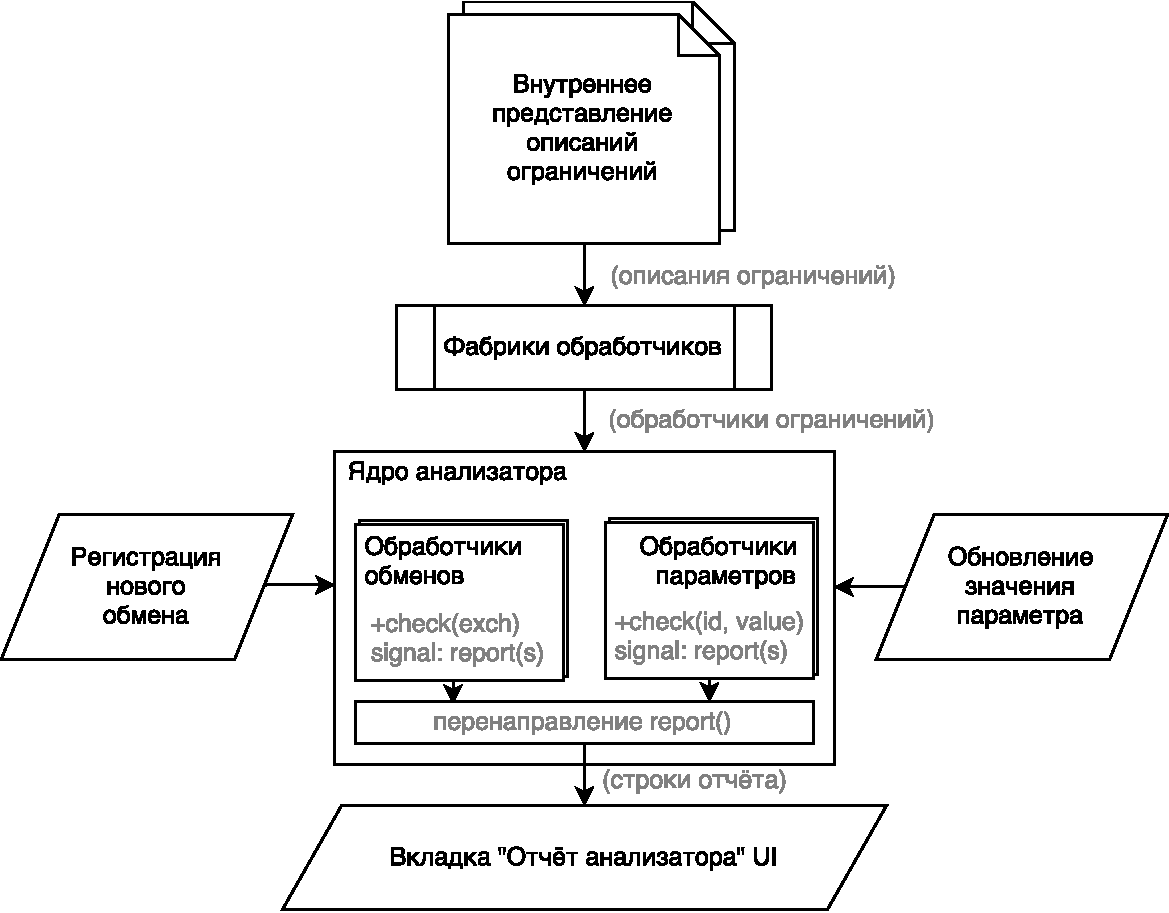
\includegraphics[scale=0.6]{base_scheme}
\caption{Общая схема архитектуры решения}
\label{figure:base_scheme}
\end{figure}

\subsection{Формат описания входных данных}
\label{sec:input_format}

\subsubsection{Общая структура файла описания}
Формат входных данных обратно совместим с форматом, использованным в некоторых 
версиях Opermon для описания сообщений и битовых полей на основе спецификации 
ПИВ.

Входные данные представляют собой XML-документ, имеющий структуру, описанную в 
листинге~\ref{input_example} в приложении~\ref{sec:listings}
% TODO: схема

Атрибуты описания абонента (тег abonent):

\begin{itemize}
 \item identifier - индентификатор абонента (строка - идентификатор Си);
 \item mil1553\_addr - адрес абонента на шине MIL STD-1553B.
\end{itemize}

Атрибуты описания параметра (тег signal):

\begin{itemize}
 \item identifier - идентификатор параметра (строка - идентификатор Си);
 \item type - тип данных параметра (например, int, unsigned int, double); 
приведён для справки;
 \item signed - является ли параметр знаковым (true|false, по умолчанию true);
 \item twosComplement - записывается ли отрицательное значение в 
дополнительном коде (true|false, по умолчанию false для совместимости со 
старым форматом ПИВ).
\end{itemize}

Тег restrict также может содержать элементы внутри, если это требуется для 
определённого типа ограничений.

Атрибуты сообщения MIL STD-1553B для контроллера (тег mil1553\_contrMessage):

\begin{itemize}
 \item identifier - идентификатор параметра (строка - индентификатор Си);
 \item direction - направление (input | output - к/от контроллера);
 \item addr  - адрес ОУ (число от 1 до 31);
 \item subaddr - подадрес ОУ (целое число от 1 до 30);
 \item numWords - число слов в сообщении (от 1 до 32).
\end{itemize}

Атрибуты сообщения MIL STD-1553B для оконечного устройства (тег 
mil1553\_termMessage):

\begin{itemize}
 \item identifier - идентификатор параметра (строка - индентификатор Си);
 \item direction - направление (input | output - к/от контроллера);
 \item subaddr - подадрес ОУ (целое число от 1 до 30);
 \item numWords - число слов в сообщении (от 1 до 32).
\end{itemize}

Стоит заметить, что в описании сообщений MIL STD-1553B для оконечных устройств 
не указан адрес ОУ-получателя сообщения. Это связано с особенностями 
внутреннего устройства используемых БД ПИВ. Для формирования полного заголовка 
сообщения требуется найти два ``полусообщения'' - сообщения 
mil1553\_termMessage у двух абонентов, где атрибуты identifier для сообщений 
совпадают.

Атрибуты описания ограничений для параметра (тег restrict внутри тега bitfield):

\begin{itemize}
 \item type - тип ограничения (см. раздел~\ref{subsec:param_restricts});
 \item value - значение для ограничения (необязательный параметр), зависит от 
типа ограничения;
 \item level - уровень критичности ограничения (info, notice, warning, error).
\end{itemize}

\subsection{Внутреннее представление конфигурации анализатора}
\label{subsec:inner}

Пользователь передаёт анализатору данные о накладываемых ограничениях в составе 
файла описания протокола. При загрузке этого описания происходит преобразование 
данных во \textit{внутреннее представление}, более пригодное для хранения в ОЗУ 
и с возможностью быстрого удобного доступа к отдельным элементам описания. При 
этом, внутреннее представление не содержит никакой информации, которую нельзя 
получить только из файла описания (взаимно однозначное соответствие описания и 
его внутреннего представления).

Внутреннее представление описания конфигурации анализатора - это пара массивов 
$A_{exch}, A_{param}$, содержащих пары \textit{(идентификатор\_объекта, 
список\_ограничений)}. Здесь идентификатор объекта - набор признаков 
конкретного типа обмена или параметра, по которым объект однозначно 
определяется в системе. Массив $A_{exch}$ содержит описания ограничений для 
обменов, $A_{param}$ - для параметров. 

Список ограничений - это массив, содержащий внутренние представления описаний 
ограничений, накладываемых на конкретный обмен или параметр. 

Внутреннее представление отдельного ограничения - это структрура данных, 
которая имеет следующий набор полей данных:

\begin{itemize}
 \item тип ограничения - один из элементов множества допустимых ограничений для 
заданного типа объекта;
 \item уровень критичности нарушения - элемент из множества уровней критичности 
нарушения ограничения \textit{(Info, Notice, Warning, Error)};
 \item значение ограничения - поле, хранящее значение атрибута value для 
данного ограничения;
 \item список дополнительных параметров - набор пар \textit{(имя\_параметра, 
значение\_параметра)}. Набор допустимых имён и значений конкретных параметров 
задан отдельно для каждого типа ограничения.
\end{itemize}

Необходимость использования общего формата описания ограничений диктуется 
требованиями простоты и расширяемости: у программиста не должно возникнуть 
необходимости в редактировании средства загрузки параметров при добавлении 
новых типов ограничений.

% TODO: типа-типа
При преобразовании данных из текстового представления во внутреннее 
представление, значения неперечисляемых типов должны сохраняться в поле 
специального типа, допускающего последующее преобразование к различным машинным 
типам данных (как минимум, к целочисленным, строковым и значениям с плавающей 
точкой). Это диктуется требованием к расширяемости, так как обработчики 
конкретных ограничений должны иметь возможность использовать данные из описания 
конфигурации любым необходимым образом. В библиотеке инструментария Qt для 
хранения таких данных предложен специальный тип QVariant.

\subsection{Получение требуемых данных}

В данном разделе рассмытриваются способы получения новых 
зарегистрированных обменов и значений параметров в рамках архитектуры 
актуальной версии Анализатора MIL STD-1553B, а конкретно - в рамках архитектуры 
компонента tabexchange, реализующего функционал, необходимый для обработки и 
отображения обменов и параметров.

\subsubsection{Получение новых обменов}

В tabexchange есть множество объектов, получающих уведомления при 
регистрации новых обменов. Соответственно, для получения анализатором 
информации о новых обменах требуется такой объект, который будет 
передавать информацию о новых обменах непосредственно анализатору.

% TODO
Уведомления рассылаются с помощью вызова виртуального метода addExchange() у 
каждого из таких объектов при регистрации нового обмена.

\subsubsection{Получение новых значений параметров}

В актуальной версии tabexchange не было реализовано функционала для рассылки 
уведомлений о получении новых значений параметров. Значения параметров 
запрашивались порциями по сигналу от внешних таймеров. Этого функционала вполне 
достаточно для реализации отображения значения параметра в соответствующей 
вкладке, а также для построения графиков зависимости значения параметра от 
времени. 

Тем не менее, для анализатора требований требуется получение 
информации о новых значениях параметра сразу после получения этого значения из 
отдельного обмена. Поэтому в рамках данной работы был изменён и 
дополнен класс, реализующий хранение и подсчёт значений параметров при 
регистрации нового обмена (с полным сохранением уже существовавшего 
функционала).

В дополнение к существующим полям, в класс был добавлен \textit{фильтр 
оперативно наблюдаемых параметров} - массив, содержащий идентификаторы 
параметров, при изменении значений которых требуется рассылка уведомлений.

При получении нового значения параметра из этого списка, происходит рассылка 
уведомления всем объектам-наблюдателям. Здесь уведомления рассылаются 
с использованием механизма ``сигнал-слот'', реализованного в инструментарии Qt 
[\ref{blanshet_qt4}].

Обновление фильтра оперативно наблюдаемых параметров происходит при загрузке 
новых описаний ограничений.


\subsection{Обработка данных}

\subsubsection{Обработчик ограничения}

Обработчик ограничения - объект специального типа, задача которого - проверять 
очередной поступивший обмен (очередное значение параметра) на корректность.

%TODO перефраз
Обработчик ограничения должен иметь метод \textit{check()}, который вызывается 
при регистрации очередного обмена (очередного значения параметра) типа, 
соответствующего данному обработчику согласно описанию ограничений. В случае 
возникновения ошибки анализа, обработчик посылает уведомление 
\textit{report()}, передавая в качестве аргумента указатель на объект строки 
отчёта, содержащей собственно сообщение об ошибке, уровень критичности ошибки и 
(опционально) ссылку на объект обмена, появление которого спровоцировало ошибку.

Отправка уведомления происходит с использованием механизма ``сигнал-слот'', 
реализованного в инструментарии Qt.

\subsubsection{Ядро анализатора}

Ядро анализатора - объект специального типа, задача которого заключается в 
распределении событий о регистрации новых обменов / новых значений параметров 
между отдельными обработчиками, а также перенаправлении уведомлений о 
возникновении ошибок от обработчиков к другим получателям (это сделано для 
инкапсуляции, чтобы не усложнять граф внешних связей анализатора).

Ядро хранит массивы пар \textit{(ключ\_объекта, список\_обработчиков)} 
отдельно для обменов и параметров. Ключ объекта здесь - значение, которое 
возможно получить или вычислить из описания зарегистрированного обмена 
(параметра), при этом позволяющее провести быстрый поиск нужного списка 
обработчиков среди всех пар (например, с применением двоичного дерева поиска - 
тогда ключи объектов должны быть сравниваемыми, или с применением хэш-таблицы - 
тогда ключи объектов должны быть хешируемыми).

Ядро анализатора имеет методы для реакции на события ``регистрация нового 
обмена'' (\textit{addExchange()}) и ``обновление значения параметра''. При 
возникновении этих событий, ядро анализатора вызывает метод \textit{check()} 
для 
всех обработчиков данного обмена (параметра), проведя поиск требуемого списка 
среди всех пар по идентификатору полученного объекта. Таким 
образом гарантируется, что обработчик будет получать на вход только те обмены 
или параметры, которые соответствуют описанию ограничения, что упрощает 
написание кода обработчика и ускоряет работу всего анализатора 
(исключаются бесполезные вызовы обработчиков).

При добавлении очередного ограничения, ядро анализатора запрашивает у фабрики 
обработчиков очередной объект и помещает его в соответствующий список 
обработчиков, а также привязывает сигнал \textit{report()} обработчика с 
собственным слотом для перенаправления. Важно заметить, что привязка сигнала 
происходит с флагом UniqueConnection, чтобы исключить привязывание сигнала 
одного и того же обработчика несколько раз (что может возникнуть при добавлении 
группового обработчика).

При удалении ограничения, ядро удаляет соответствующий элемент из списка и 
отвязывает сигнал report().

\subsubsection{Фабрика обработчиков}

Для создания обработчиков используется специальный объект-фабрика [\ref{gof}]. 
Фабрика в данном случае позволяет решить сразу две проблемы: она позволяет 
создавать объекты различных типов по текстовому описанию имени, а также следит 
за необходимостью создания объектов отдельных типов. Например, при 
конфигурировании обработчика ограничения на связанность значений параметров, 
объект обработчика требуется создавать только для новых имён групп; если 
запрашивается обработчик для группы, определённой ранее, фабрика вернёт 
указатель на ранее созданный объект.

Таким образом, например, для обработчиков групп связанных параметров, фабрика 
должна хранить массив пар \textit{(идентификатор\_группы, обработчик)}. Для 
того, чтобы уже созданный обработчик узнал о существовании ещё одного параметра 
в группе, фабрика при запросе объекта вызывает у нужного обработчика метод 
\textit{attach()}, принимающий в качестве аргумента ссылку на внутреннее 
представление очередного ограничения.

Создание обработчика происходит явным вызовом метода-конструктора, принимающего 
в качестве аргумента ссылку на внутреннее представление ограничения.

\subsection{Передача результатов проверки}

По результатам проверки, обработчик отдельного ограничения может оповестить 
систему о возникновении ошибки (или не оповестить, если ошибки обнаружено не 
было). Оповещение происходит в рамках выполнения метода \textit{check()} 
обработчика ограничения.

Для оповещения используется механизм ``сигнал-слот'', реализованный в 
инструментарии Qt.

На оповещения от ядра анализатора подписан объект модели таблицы отчёта 
анализатора. При получении оповещения, новое сообщение об ошибке добавляется в 
список строк таблицы, после чего запрашивается перерисовка пользовательского 
интерфейса. Таким образом, реализуется возможность использования анализатора при 
регистрации обменов в режиме реального времени.